\section{Introduction}

Programming languages researchers have developed a variety of tools and methods for helping programmers and users understand their programs, ranging from provenance techniques and taint tracking to dataflow analysis and program slicing. These tools have a wide range of applications, including security, optimisation and program comprehension. An increasingly important problem, particularly in data science and scientific computing where transparency and reproducibility are paramount, is understanding how programs transform richly structured inputs into richly structured outputs. Visualisation code turns tables of data into charts and other graphics; array computations operate on large multidimensional structures; compilers turn abstract syntax trees into compiled code. For problem domains such as these, we need analysis tools that let us focus on a particular part of the output to see what parts of the input contribute to it, as well as to see what part of the input affects what part of the output. \todo{Some evidence that we need this.}

[SKETCH OF A NEW VERSION]

The problem of relating structured outputs to structured inputs is ubiquitous and particularly pressing in data visualisations. To make data visualizations more understandable, journalists, scientists and policy makers increasingly want to create charts that let the user see how aspects of the visual output relate to input data as well as other charts generated from the same input data. From a program analysis perspective, there are two interesting problems. In the first problem, we want to be able to select a visual element and see what input data contribute to it. This is a matter of focusing on a part of the structured output and performing a backwards analysis that propagates information through the program and highlights parts of the input data as well as parts of the program that contribute to the output. In the second, more challenging problem, we want to understand how two charts produced from the same data relate. We want to be able to select a visual element in one output chart and see what aspects of a different chart are computed using related inputs. This is a matter of focusing on a part of the structured output, performing backwards analysis to parts of program and data that contribute to it, but then also performing forwards analysis to highlight related parts of the other output.

In this case, we need a more sophisticated approach that supports both backwards and forwards analysis. Furthermore, to guarantee desirable properties of the analysis (which ones?) the two analyses have to be related through a desirable theoretical connection.

[ORIGINAL VERSION]

One area where this is particularly important is data visualization. Journalists, scientists and policy makers use data visualization to turn input data into visual summaries, but charts can be hard to intepret correctly. A key part of understanding and trusting a visualization means knowing what data the visual attributes actually represent. To address this, much work in data visualization has been done to assist analysts understand the mapping between data source and visual elements in the visualization and understand how different views of the same data are related. This is typically done through data visualization lirbaries that do not utilize rich program analysis techniques.

[TODO: Talk more about the motivation for linking and the existing libraries for this.]
However, because data visualization libraries cannot analyze the host language, they resort to using internal DSLs where normal data transformation is encoded not as normal host language calculations, but as operations in the DSL. Wouldn't it be nice if we could write code to produce data visualization in a standard programming language and then be able to question how the structured output relates to structured inputs using a clever PL technique? For example, consider the following linked visualization example (Figure X):

let data = [ ... ]
let barchart = data |> some transformation
let linechart = data |> some other transformation

Here, the code is written in normal programming language. The technique presented in this paper makes it possible to auotmatically link the barchart to the linechart. This is done by propagating information backwards, from the barchart to the data and then forwards, from the data to the linechart. Moreover, our method has nice theoretical properties, meaning that (some good things).

\section{Introduction}

Data, curated by journalists, scientists and policy makers into charts and other visual summaries, is how we understand the changing world around us. But charts can be hard to interpret correctly, even with access to the relevant data source. Innocent (but devastating) mistakes such as transposing two columns of data may go unnoticed for several years, even in widely cited papers~\cite{miller06}. Less innocent mistakes are deployed by politicians to mislead voters~\cite{fullfact19}. Understanding and trusting a visualisation, even for an expert, means knowing what its visual attributes actually \emph{represent}, which in turn involves the following two comprehension challenges:

\begin{enumerate}
  \item Identifying the mapping between data source and visual elements in the visualisation
  \item Understanding how different views of the same data are related
\end{enumerate}

\noindent Even with the data and source code used to create the visualisation to hand, answering questions such as these is difficult, requiring time and expertise. The basic problem is that visualisations are opaque, disconnected from the data and computations used to create them. This situation would be significantly imporved if visualisations allowed a reader to explore the relationship to the underlying data through the visualisation itself, revealing the relevant connections on a need-to-know basis, as the reader interacts with it (\figref{introduction:data-linking} below):

\begin{figure}[H]
   {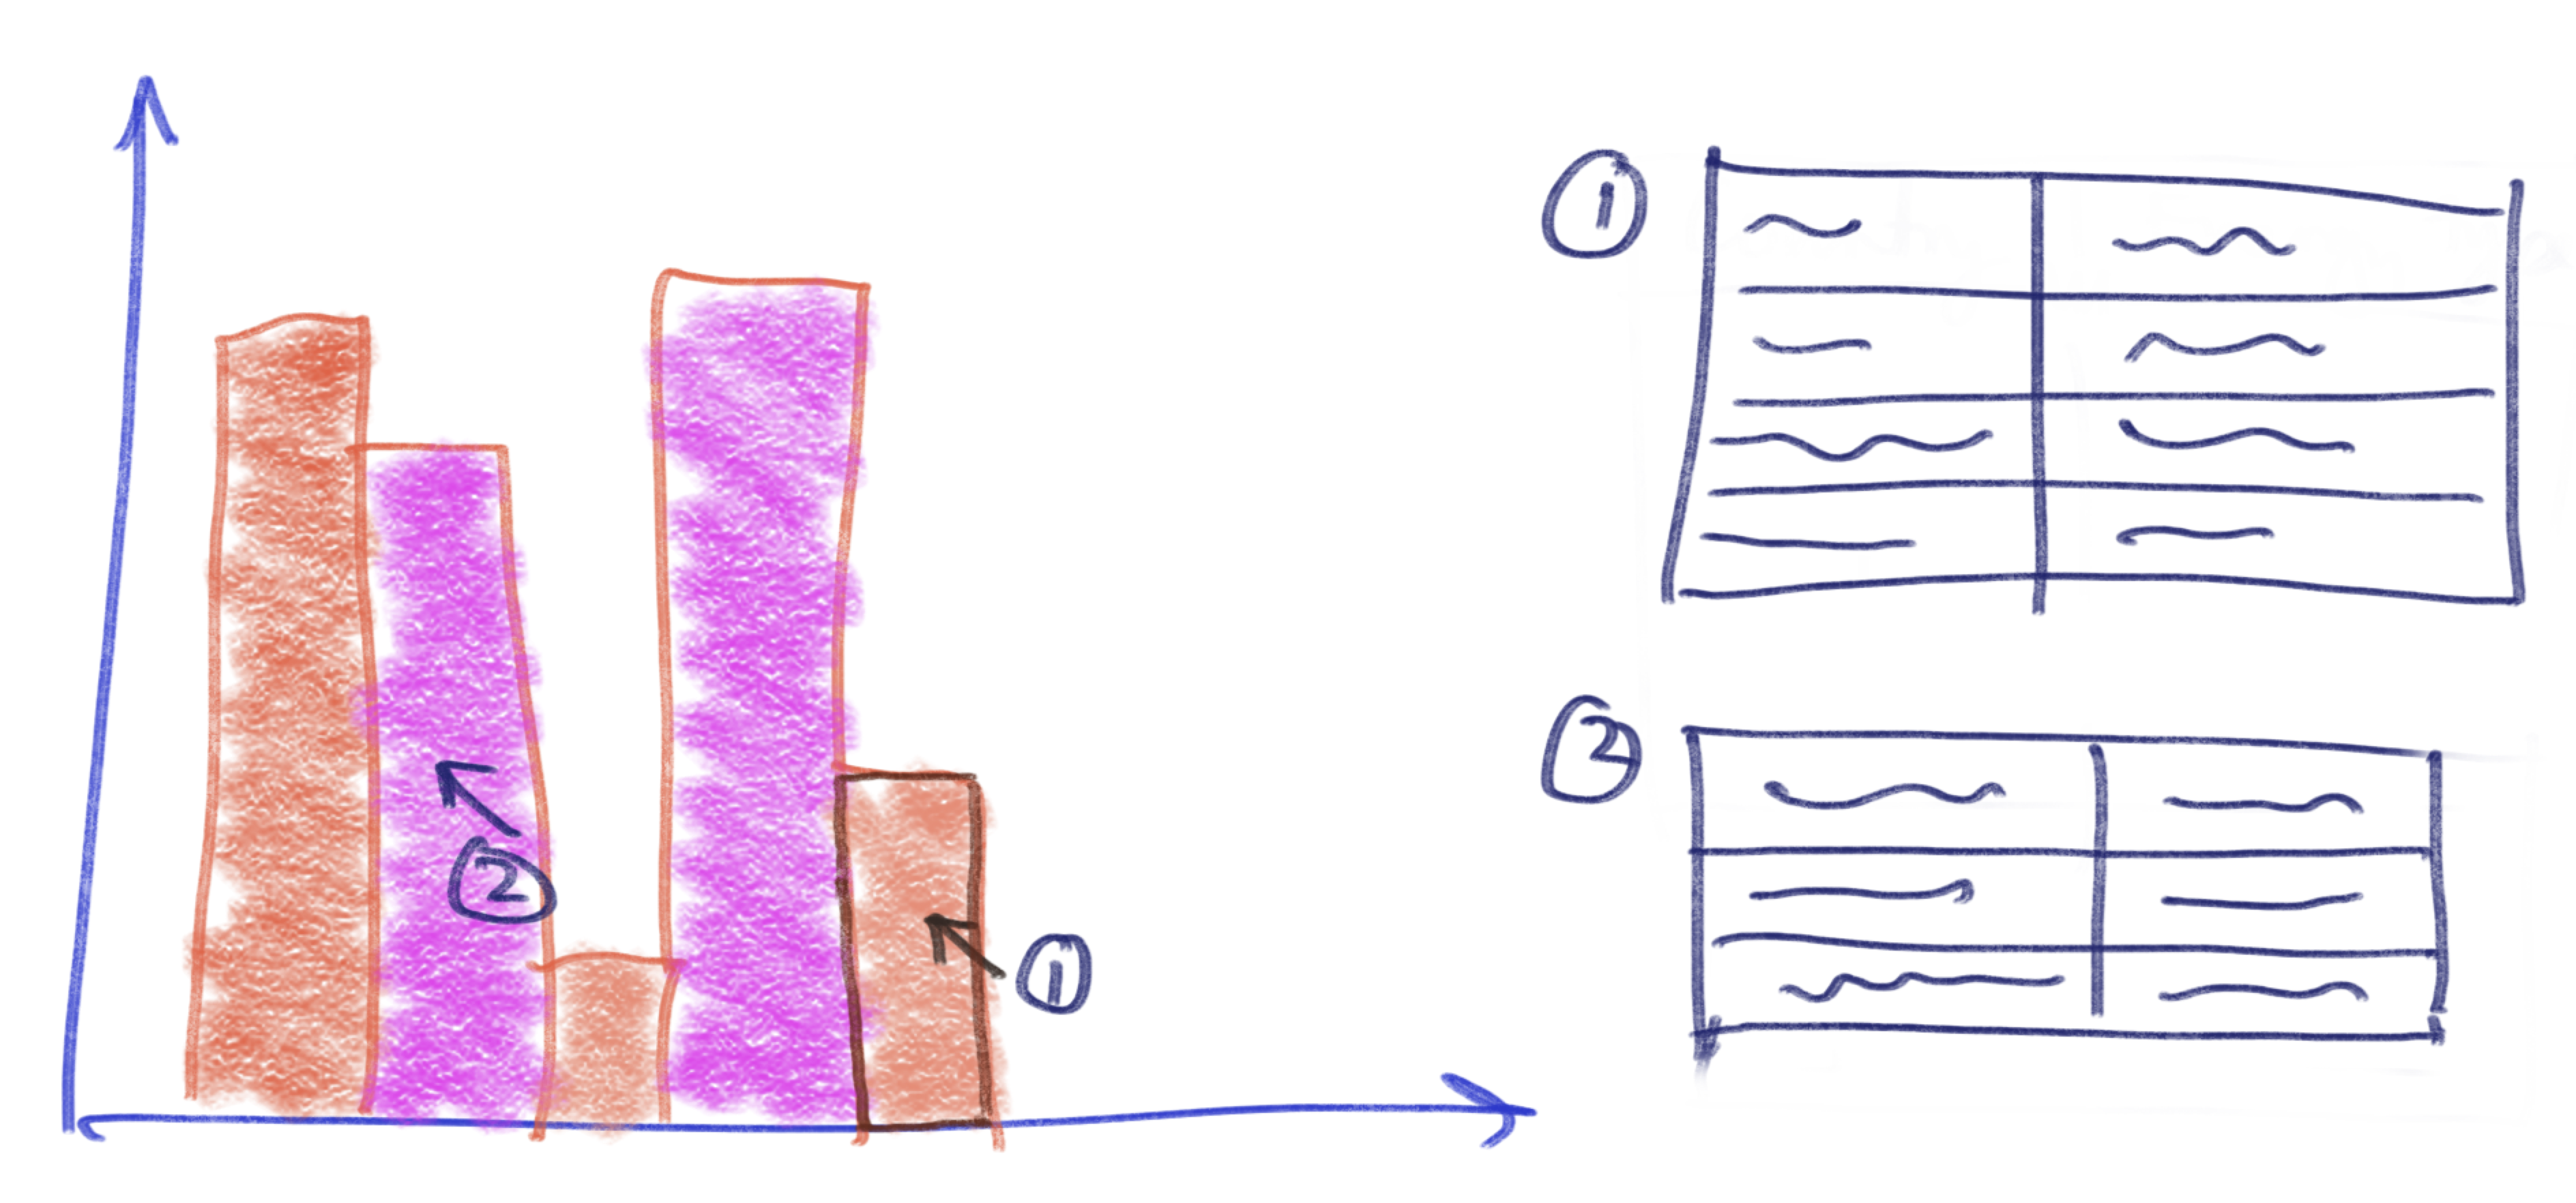
\includegraphics[scale=0.07]{fig/example/data-linking.png}}
   \caption{Data visualisation with fine-grained data linking}
   \label{fig:introduction:data-linking}
\end{figure}

Building this sort of ``data-linked'' visualisation by hand is possible, but is a significant undertaking, requiring intimate knowledge of the computational relationship between chart and data, and programming effort to expose that information to the reader. Manual approaches are also unlikely to be correct and lead to brittle solutions that need to be changed whenever the application logic changes. Given that a visualisation is a view computed from a data source, it seems plausible that we might adapt techniques from program analysis and data provenance to provide a runtime infrastructure that automatically supports linked selections. Then the data scientist or visualisation designer can concern themselves with cleaning, aggregating and presenting data, leaving the infrastructure to take care of linking visualisations to the underlying data sources.

\subsection{Linking visualisations to each other}

It is also common to use more than one view to present distinct but related aspects of data. (We say visualisations are \emph{cognate} when they are related in this way.) Geospatial applications like GeoDa~\cite{anselin06} and charting libraries like Plotly provide a view coordination feature called \emph{brushing and linking}~\cite{becker87}, where selections in one chart automatically select corresponding elements in the other, as an aid to comprehension. In \figref{introduction:vis-linking} below, selecting a bar on the left automatically selects all the related visual elements on the right. Although such coordination features are highly desirable, they are either baked into specific applications, or require programmer effort and therefore must be anticipated in advance by the chart designer. Moreover the linking is opaque, providing no direct way for the reader to see the data which underpins the relationship.

\begin{figure}[H]
   {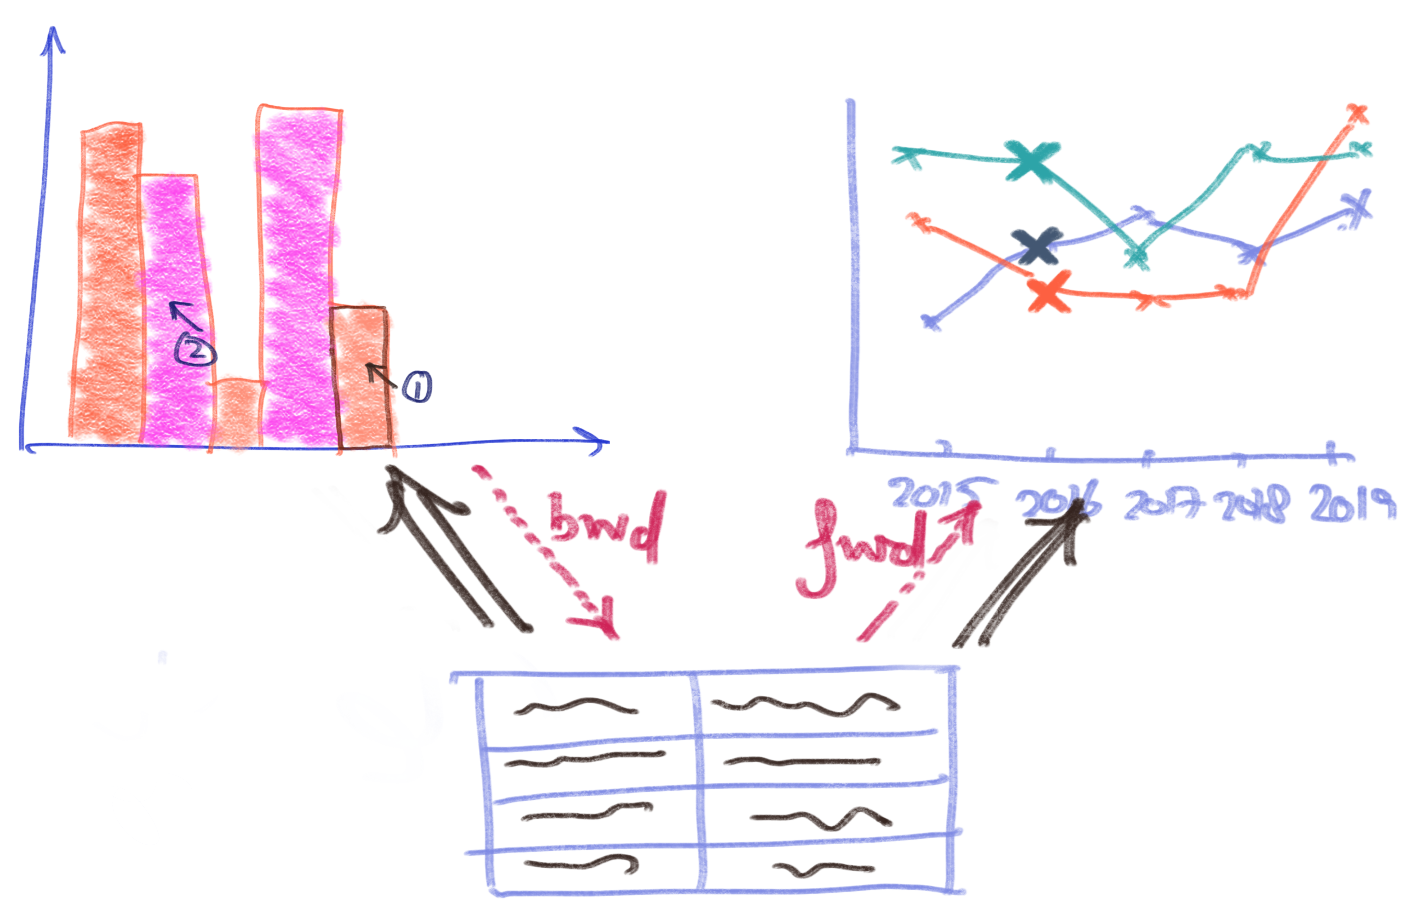
\includegraphics[scale=0.14]{fig/example/vis-linking.png}}
   \caption{Linking cognate visualisations via common data dependencies}
   \label{fig:introduction:vis-linking}
\end{figure}

\subsection{Our contributions}

In this paper, we present new language-based data provenance techniques for linking visualisations to data, and to each other, in a fine-grained way. Our specific contributions are as follows:

\begin{itemize}[leftmargin=*]
   \item[--] a review of \emph{Galois slicing}, a program slicing framework with round-tripping properties appropriate to our problem, and an analysis of its shortcomings (\secref{background});
   \item[--] a new bidirectional dependency analysis inspired by Galois slicing, addressing these shortcomings, for a core calculus with lists and arrays, and a discussion of how the components of this analysis can be combined in various ways to link inputs to outputs and outputs to other outputs (\secref{core-language});
   \item[--] a richer surface language called \OurLanguage with familiar functional programming features, including piecewise definitions, pattern matching, list notation and list comprehensions, and an extension of our analysis to the desugaring (\secref{surface-language});
   \item[--] an implementation of Fluid in PureScript, and a discussion and evaluation of the strengths and weaknesses of our approach (\secref{implementation}).
\end{itemize}
